\documentclass{standalone}
\usepackage{tikz}
\usepackage{ctex,siunitx}
\setCJKmainfont{Noto Serif CJK SC}
\usepackage{tkz-euclide}
\usepackage{amsmath}
\usetikzlibrary{patterns, calc}
\usetikzlibrary {decorations.pathmorphing, decorations.pathreplacing, decorations.shapes,}
\begin{document}
\small
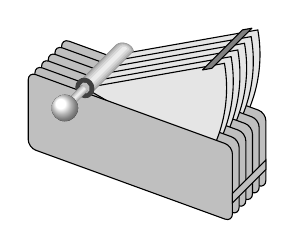
\begin{tikzpicture}[>=stealth,scale=1.2]
  \foreach \x[count=\i] in {0.5,0.4,0.3,0.2,0.1,0.0}
  {
    \draw[fill=lightgray!40](45:\x)--++(10:1.5)arc(10:-30:1.5)--cycle;
    \draw[fill=lightgray,rounded corners=1mm](45:\x-0.05)--++(-20:1.7)--++(0,-0.8)coordinate (A\i)--++(160:2.3)--++(0,0.8)--cycle;
  }
  \draw[fill=gray,line join=round](10:1.4)--++(45:0.55)--++(190:0.1)--++(225:0.6)--++(10:0.1)--cycle;
  \foreach \x in {90,75,60,45,30,15}
  {
    \fill[gray!\x](0,0)--++(160:{0.1*sin(\x)})--++(45:0.6)to[bend left=60]++(-20:{0.2*sin(\x)})--++(225:0.6)--cycle;
  }
  \fill[darkgray,rotate=20](0,0)ellipse(0.1 and 0.11);
  \fill[lightgray,rotate=20](0,0)ellipse(0.05 and 0.06);
  \foreach \x in {90,75,60,45,30,15}
  {
    \draw[line width={3*sin(\x)},gray!\x](0,0)--(225:0.3);
  }
  \fill[ball color=white](225:0.3)circle(4pt);
  \draw[fill=lightgray]([yshift=0.2cm]A1)--++(225:0.5)--++(0,0.1)--++(45:0.5)--cycle;
\end{tikzpicture}
\end{document}